%-------------------------------------------------------------------------------
%                                PREAMBLE
%-------------------------------------------------------------------------------
\documentclass[usenames,dvipsnames,svgnames,10pt,aspectratio=169]{beamer}
\usefonttheme{professionalfonts}

% This theme uses TIKZ: compile twice with PDFLaTeX or LuaLaTeX.
%
%  Options:
%  - [clean]:    clean slides, i.e. logos and footbar are removed
%  - [kth]:      footbar style inspierd to the official KTH template
%  - [nicewave]: a different style of wave is used (not approved by FLOW)
%
\usetheme{flow}

\usepackage{hyperref,graphicx,lmodern}
\usepackage[utf8]{inputenc}
\usepackage{media9}
\usepackage{xcolor}
\usepackage{stmaryrd}
\usepackage{nicefrac}
\usepackage{multimedia}
\usepackage{multicol}
\usepackage{upgreek}
\usepackage[]{bm}
\usepackage[]{url}

\graphicspath{{imgs/}}
\setbeamertemplate{blocks}[rounded][shadow=true]


\DeclareMathOperator{\trace}{tr}

%-------------------------------------------------------------------------------
%                                TITLE PAGE
%-------------------------------------------------------------------------------
\title[Nonlinear Physics] % Short title used in footline
{
	Nonlinear physics, dynamical \\ systems and chaos theory
}

\author[J.-Ch.~Loiseau] % Presenting author in short form used in footline
{
	Jean-Christophe Loiseau
}
% - Give the names in the same order as the appear in the paper.
% - Underline the presenting author.

\institute[unused]
{
	\url{jean-christophe.loiseau@ensam.eu} \\
	DynFluid, \\
	Arts et M\'etiers ParisTech, France
}
% Keep it simple, no one is interested in your street address.

% University logo(s)
\logot{
\includegraphics[width=.128\paperwidth]{DynFluid_logo}}  % Top logo
\logob{
\includegraphics[width=0.128\paperwidth]{ENSAM_logo}} % Bottom logo
% \logoc[{
\includegraphics[width=.128\paperwidth]{limsi}}]{
\includegraphics[width=.128\paperwidth]{limsi}} % Corner logo
%
% Cover image: \cvrimg{x position}{y position}{cover image}
\cvrimg{.77}{.8}{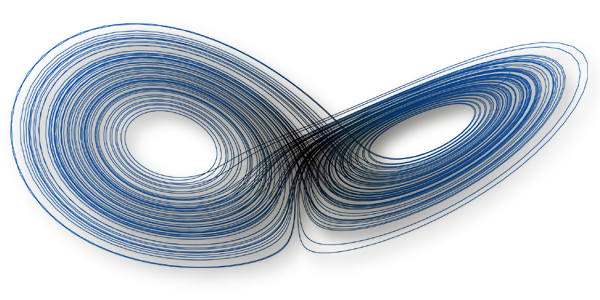
\includegraphics[width=.4\paperwidth]{cover.png}}

\date[unused]{ENSAM, Master 2, 2018--2019}

\begin{document}

\titleframe % Print the title as the first slide

%-------------------------------------------------------------------------------
%                           PRESENTATION SLIDES
%-------------------------------------------------------------------------------

\begin{frame}[t, c]{}
	\centering
	\vspace{1cm}

	{\Large \textbf{First-order systems}}

	\bigskip

	{\textgre{\textbf{Flows on the line}}}

\end{frame}

\begin{frame}[t, c]{First-order systems}{An apparently simple system}
	\begin{itemize}
		\item Let us consider the following first-order dynamical system
		$$
		\dot{x} = \sin(x).
		$$

		\bigskip

		\item Its analytical solution is given by
		$$
		t = \displaystyle \ln \left\vert \frac{\csc(x_0) + \cot(x_0)}{\csc(x) + \cot(x)} \right\vert.
		$$
	\end{itemize}

	\vspace{1cm}
\end{frame}

\begin{frame}[t, c]{First-order systems}{Phase line}
	\centering

	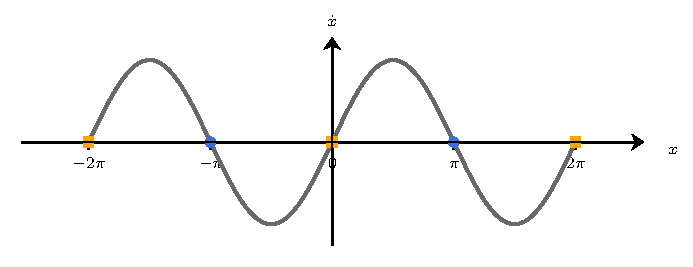
\includegraphics[width=.75\textwidth]{flow_on_the_line}

	\bigskip

	Phase line of the first-order dynamical system considered.

	\vspace{1cm}
\end{frame}

\begin{frame}[t, c]{First-order systems}{Fixed points}
	\begin{itemize}
		\item Fixed points $x^*$ are equilibrium solutions characterized by
		$$
		f(x^*) = 0.
		$$

		\bigskip

		\item In the present case, these are given by
		$$
		x^* = n \pi \text{ for } n \in \mathbb{N}.
		$$
	\end{itemize}

	\vspace{1cm}
\end{frame}

\begin{frame}[t, c]{First-order systems}{Linear stability}
	\begin{itemize}
		\item The dynamics of a perturbation $\eta(t) = x(t) - x^*$ is given by
		$$
		\dot{\eta} = f(x^* + \eta).
		$$

		\bigskip

		\item If $\eta$ is small enough, $f(x^* + \eta)$ can be approximated by its first-order Taylor expansion around $x^*$
		$$
		f(x^* + \eta) = f(x^*) + f^{\prime}(x^*) \eta + \mathcal{O}(\eta^2).
		$$
	\end{itemize}

	\vspace{1cm}
\end{frame}

\begin{frame}[t, c]{First-order systems}{Linear stability}
	\begin{itemize}
		\item Given that $f(x^*) = 0$, the dynamics of $\eta$ are governed by
		$$
		\dot{\eta} = f^{\prime}(x^*) \eta.
		$$

		\bigskip

		\item Its analytical solution is given by
		$$
		\eta(t) = \exp \left( f^{\prime}(x^*) t \right) \eta_0.
		$$
	\end{itemize}

	\vspace{1cm}
\end{frame}

\begin{frame}[t, c]{First-order systems}{Linear stability}
	\begin{itemize}
		\item The linear stability of a fixed point $x^*$ is determined by the sign of $f^{\prime}(x^*)$:

		\begin{itemize}
			\item[$\hookrightarrow$] if $f^{\prime}(x^*) > 0$, $\eta(t)$ growths exponentially fast. The fixed point is said to be \alert{\textbf{linearly unstable}}.

			\medskip

			\item[$\hookrightarrow$] if $f^{\prime}(x^*) < 0$, $\eta(t)$ decays exponentially fast. The fixed point is said to be \alert{\textbf{linearly stable}}.

			\medskip

			\item[$\hookrightarrow$] if $f^{\prime}(x^*) = 0$, one can not conclude and nonlinear analyses are required.
		\end{itemize}

		\bigskip

		\item Let us now re-analyze our original system and sketch the evolution of $x(t)$.
	\end{itemize}

	\vspace{1cm}
\end{frame}

\begin{frame}[t, c]{First-order systems}{Phase line}
	\centering

	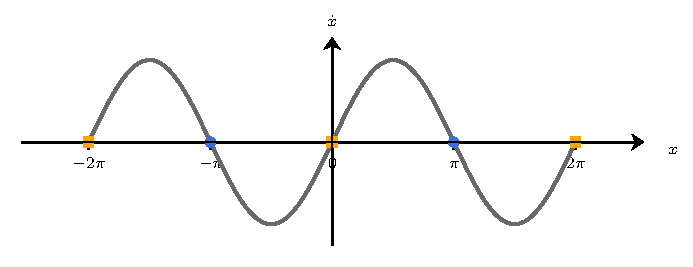
\includegraphics[width=.75\textwidth]{flow_on_the_line}

		\bigskip

		Phase line of the first-order dynamical system considered.
	\vspace{1cm}
\end{frame}

\begin{frame}[t, c]{First-order systems}{Evolution of $x(t)$}
	\centering

		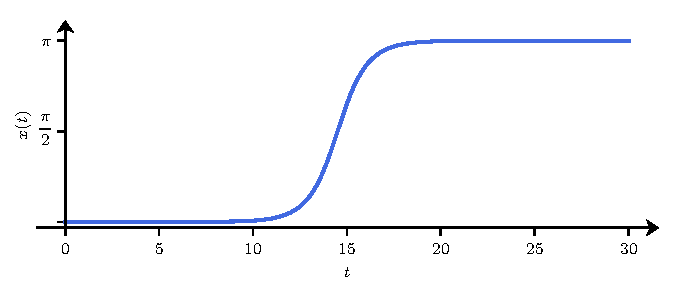
\includegraphics[width=.75\textwidth]{flow_on_the_line_bis}

		\bigskip

		Evolution of $x(t)$ for the initial condition $x_0 = 10^{-6}$.

	\vspace{1cm}
\end{frame}

\begin{frame}[t, c]{First-order systems}{}

	\centering
	\begin{block}{\centering \textbf{Warning!}}
		For a first-order system, the trajectories can only vary monotonically: either they end up on a stable fixed point, or they diverge to $\pm \infty$.
	\end{block}

	\vspace{1cm}
\end{frame}


\begin{frame}[t, c]{}
	\centering
	\vspace{1cm}

	{\Large \textbf{Second-order systems}}

	\bigskip

	{\textgre{\textbf{Oscillators, but not only...}}}

\end{frame}

\begin{frame}[t, c]{Second-order systems}{}
	\begin{itemize}
		\item Second-order systems are dynamical systems which can be described by
		\begin{equation}
			\begin{aligned}
				\dot{x} & = f(x, y) \\
				\dot{y} & = g(x, y).
			\end{aligned}
			\notag
		\end{equation}

		\bigskip

		\item Having two degrees of freedom, they can exhibit dynamics much richer than simple first-order systems.
	\end{itemize}

	\vspace{1cm}
\end{frame}

\begin{frame}[t, c]{Second-order system}{Our working example}
	\begin{itemize}
		\item For the rest of this section, let us consider the following system
		\begin{equation}
			\begin{aligned}
				\dot{x} & = x - y^2 + 1.28 + 1.4 xy \\
				\dot{y} & = 0.2 y - x + x^3.
			\end{aligned}
			\notag
		\end{equation}

		\bigskip

		\item Note that this system is considered only for illustration purposes. To the best of my knowledge, it does not model any particular physics.
	\end{itemize}

	\vspace{1cm}
\end{frame}

\begin{frame}[t, c]{Second-order systems}{Phase plane and isoclines}
	\centering

	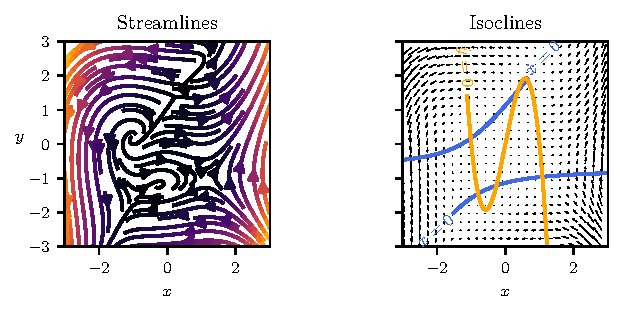
\includegraphics[width=.75\textwidth]{phase_plane_and_isoclines}

	Phase plane and isoclines (i.e. $\dot{x} = 0$ and $\dot{y} = 0$) of the system considered.

	\vspace{1cm}
\end{frame}

\begin{frame}[t, c]{Second-order systems}{Phase plane and isoclines}
	\begin{itemize}
		\item For a second-order system, phase plane and isoclines are fairly easy to plot and provide valuable insights into the dynamics of the system.
		\begin{itemize}
			\item[$\hookrightarrow$] Phase plane : general overview of the dynamics of the system.

			\item[$\hookrightarrow$] Direct visualization of the stable and unstable fixed point of the system.
		\end{itemize}
	\end{itemize}

	\bigskip

	\begin{block}{\centering \textbf{Question}}
		\centering
		How to compute these fixed points?
	\end{block}
\end{frame}

\begin{frame}[t, c]{}
	\centering
	\vspace{1cm}

	{\Large \textbf{Interlude}}

	\bigskip

	{\textgre{\textbf{How to compute fixed points?}}}

\end{frame}

\begin{frame}[t, c]{How to compute fixed points?}{Different techniques}
	\begin{itemize}
		\item Fixed points are structuring the phase space of the dynamical system under scrutiny. Unfortunately, it may not be easy (nor possible) to compute them analytically.

		\bigskip

		\item A number of different numerical techniques exist for that purpose. The following list is by no means exhaustive:
		\begin{itemize}
			\item[$\hookrightarrow$] Newton-Raphson method,
			\item[$\hookrightarrow$] Selective Frequency Damping,
			\item[$\hookrightarrow$] BoostConv,
			\item[$\hookrightarrow$] ...
		\end{itemize}
	\end{itemize}

	\vspace{1cm}
\end{frame}

\begin{frame}[t, c]{Newton-Raphson method}{$f : \mathbb{R} \to \mathbb{R}$}
	\begin{itemize}
		\item Originally proposed by Isaac Newton (1645--1727) and Joseph Raphson (1648 -- 1715) to solve
		$$f(x) = 0.$$

		\medskip

		\item Given an initial guess $x_0$, the idea is to approximate $f(x)$ by its first-order Taylor expansion around $x_0$, i.e.\
		$$
		f(x) \simeq f(x_0) + f^{\prime}(x_0) ( x - x_0).
		$$

		\medskip

		\item A better estimate $x_1$ of the root of $f$ can then be obtained by solving
		$$
		0 = f(x_0) + f^{\prime}(x_0) ( x_1 - x_0).
		$$
	\end{itemize}

	\vspace{1cm}
\end{frame}

\begin{frame}[t, c]{Newton-Raphson method}{$f : \mathbb{R} \to \mathbb{R}$}
	\begin{itemize}
		\item After $k$ iterations, the basic iteration scheme can be written as
		$$
		x_{k+1} = x_k - \displaystyle \frac{f(x_k)}{f^{\prime}(x_k)}.
		$$

		\bigskip

		\item The iterative procedure stops when a user-defined criterion is fulfilled, usually
		$$
		\| f(x_k) \| \le \epsilon \text{ or } \| x_{k+1} - x_k \| \le \epsilon,
		$$
		with $\epsilon \simeq 10^{-10}$.
	\end{itemize}

	\vspace{1cm}
\end{frame}


\begin{frame}[t, c]{Newton-Raphson method}{$f : \mathbb{R} \to \mathbb{R}$}
	\centering

	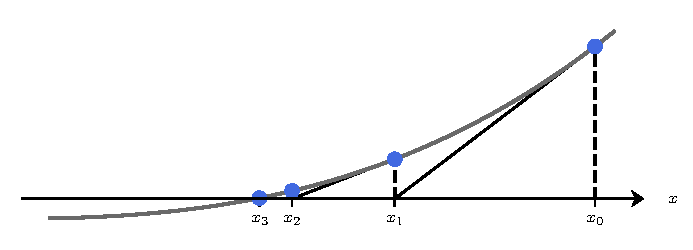
\includegraphics[width=.75\textwidth]{Newton_method}

	\bigskip

	Illustration of the Newton-Raphson for $f(x) = x^3 - 2x - 5$ and $x_0=3.8$.

	\vspace{1cm}
\end{frame}


\begin{frame}[t, c]{Newton-Raphson method}{${\bm f} : \mathbb{R}^n \to \mathbb{R}^n$}

	\begin{itemize}
		\item Generalization of the Newton-Raphson method to the case ${\bm f} : \mathbb{R}^n \to \mathbb{R}^n$ is quite straightforward.

		\bigskip

		\item Given an estimate ${\bm x}_k$, the basic iteration reads
		\begin{equation}
			\begin{aligned}
				{\bm J} \delta {\bm x} & = - {\bm f}({\bm x}_k) \\
				{\bm x}_{k+1} & = {\bm x}_k + \delta {\bm x},
			\end{aligned}
			\notag
		\end{equation}
		where ${\bm J}$ is the Jacobian matrix of ${\bm f}$ evaluated at ${\bm x}_k$.
	\end{itemize}

	\vspace{1cm}
\end{frame}

\begin{frame}[t, c]{Newton-Raphson method}{Limitations}
	\begin{itemize}
		\item Although efficient, Newton-Raphson method suffers from a number of limitations:
		\begin{itemize}
			\item[$\hookrightarrow$] The fixed points computed may depend on the initial guess ${\bm x}_0$.
			\item[$\hookrightarrow$] Evaluating ${\bm f}({\bm x})$ might be computationally expensive.
			\item[$\hookrightarrow$] At each iteration, the Jacobian matrix ${\bm J}$ needs to be evaluated and inverted ($\mathcal{O}(n^3)$ operations).
		\end{itemize}

		\bigskip

		\item A number of variants of the Newton-Raphson method exist as to address these different limitations. This however is algorithmic refinement beyond the scope of the present course.
	\end{itemize}

	\vspace{1cm}
\end{frame}


\begin{frame}[t, c]{}
	\centering
	\vspace{1cm}

	{\Large \textbf{Second-order systems}}

	\bigskip

	{\textgre{\textbf{Back to our example}}}

\end{frame}

\begin{frame}[t, c]{Second-order systems}{Fixed point computation}
	\begin{itemize}
		\item Visual inspection of the isoclines has revealed that the system exhibits six different fixed points.

		\bigskip

		\item In the rest, we will use the Newton-Raphson method to compute these different fixed points.

		\bigskip

		\item The state-dependent Jacobian matrix required for Newton method reads
		\begin{equation}
			{\bm J} = \begin{bmatrix}
									1 + 1.4y & -2 y + 1.4 x \\
									-1 + 3 x^2 & 0.2
								\end{bmatrix}
			\notag
		\end{equation}
	\end{itemize}

	\vspace{1cm}
\end{frame}

\begin{frame}[t, c]{Second-order systems}{Infinitesimal perturbations}
	\begin{itemize}
		\item The dynamics of an infinitesimal perturbation ${\bm q}$ evolving in the vicinity of a given fixed point ${\bm x}^*$ is given by
		$$\dot{\bm q} = {\bm L}{\bm q},$$
		where ${\bm L}$ is the Jacobian matrix of the system evaluated at ${\bm x} = {\bm x}^*$.

		\bigskip

		\item The analytical solution to this \alert{\textbf{linear time-invariant dynamical system}} is given by
		$${\bm q}(t) = e^{{\bm L}t}{\bm q}_0,$$
		where ${\bm q}_0$ is the initial condition.
	\end{itemize}

	\vspace{1cm}
\end{frame}

\begin{frame}[t, c]{}
	\centering
	\vspace{1cm}

	{\Large \textbf{Interlude}}

	\bigskip

	{\textgre{\textbf{Some elements of linear algebra}}}

\end{frame}

\begin{frame}[t, c]{Some elements of linear algebra}{Matrix decompositions}
	Stewart (\emph{Comput. Sci. Engrg.}, \textbf{2}:50--59, 2000) has listed the \emph{big six matrix decompositions}:


	\begin{enumerate}
		\item Cholesky decomposition,
		\item Pivoted LU decomposition,
		\item QR decomposition,
		\item Spectral decomposition, also known as \alert{\textbf{Eigendecomposition}},
		\item Schur decomposition,
		\item Singular Value decomposition.
	\end{enumerate}

	\vspace{1cm}
\end{frame}

\begin{frame}[t, c]{Some elements of linear algebra}{Eigendecomposition of a matrix}
	\begin{itemize}
		\item Eigendecomposition is the factorization of a matrix into its canonical form.
		\begin{itemize}
			\item[$\hookrightarrow$] The matrix is represented in terms of its \alert{\textbf{eigenvalues}} and \alert{\textbf{eigenvectors}}.
		\end{itemize}

		\bigskip

		\item Given a $n \times n$ (i.e.\ square) matrix ${\bm L}$, eigendecomposition aims to rewrite it as
		$${\bm L} = {\bm V} {\boldsymbol \Lambda}{\bm V}^{-1},$$
		where ${\boldsymbol \Lambda}$ is the diagonal matrix of \alert{\textbf{eigenvalues}} and ${\bm V}$ is a $n \times n$ matrix whose i\textsuperscript{th} column if the \alert{\textbf{eigenvector}} ${\bm v}_i$ associated to ${\boldsymbol \Lambda}_{ii} = \lambda_i$.
	\end{itemize}

	\vspace{1cm}
\end{frame}

\begin{frame}[t, c]{Some elements of linear algebra}{Matrix exponential}

	\begin{block}{\centering \textbf{Warning, unless the matrix is diagonal,}}
		\begin{equation}
			\left( e^{\bm L} \right)_{ij} \neq e^{l_{ij}}
			\notag
		\end{equation}
	\end{block}

	\vspace{1cm}
\end{frame}

\begin{frame}[t, c]{Some elements of linear algebra}{Matrix exponential}
	\begin{itemize}
		\item The infinitie series Taylor expansion of the classical exponential function $f(x) = e^x$ is given by
		$$f(x) = 1 + x + \displaystyle \frac{x^2}{2!} + \frac{x^3}{3!} + \cdots$$

		\bigskip

		\item The same definition carries over for matrices.
		$$e^{\bm L} = {\bm I} + {\bm L} + \displaystyle  \frac{{\bm L}^2}{2!} + \frac{{\bm L}^3}{3!} + \cdots,$$
		where ${\bm I}$ is the identity matrix.
	\end{itemize}

	\vspace{1cm}
\end{frame}

\begin{frame}[t, c]{Some elements of linear algebra}{Matrix exponential}
	\begin{itemize}
		\item Evaluating $e^{\bm L}$ by brute force is quite impractical and extremely expansive from a computational point of view.

		\bigskip

		\item Using the eigendecomposition of ${\bm L}$, the matrix exponential can be rewritten as
		$$e^{\bm L} = {\bm V} e^{\boldsymbol \Lambda} {\bm V}^{-1},$$
		where $e^{\boldsymbol \Lambda}$ can easily be evaluated as it is a diagonal matrix.
	\end{itemize}

	\vspace{1cm}
\end{frame}

\begin{frame}[t, c]{Some elements of matrix algebra}{Matrix exponential}
	\begin{equation}
		\begin{aligned}
			e^{\bm L} & = {\bm I} + {\bm L} + \displaystyle \frac{{\bm L}^2}{2!} + \frac{{\bm L}^3}{3!} + \cdots, \\
			& = {\bm I} + {\bm V}{\boldsymbol \Lambda}{\bm V}^{-1} + \displaystyle \frac{{\bm V}{\boldsymbol \Lambda}{\bm V}^{-1}{\bm V}{\boldsymbol \Lambda}{\bm V}^{-1}}{2!} + \frac{{\bm V}{\boldsymbol \Lambda}{\bm V}^{-1}{\bm V}{\boldsymbol \Lambda}{\bm V}^{-1}{\bm V}{\boldsymbol \Lambda}{\bm V}^{-1}}{3!} + \cdots, \\
			& = {\bm V}{\bm I}{\bm V}^{-1} + {\bm V}{\boldsymbol \Lambda}{\bm V}^{-1} + \displaystyle \frac{{\bm V}{\boldsymbol \Lambda}^2{\bm V}^{-1}}{2!} + \frac{{\bm V}{\boldsymbol \Lambda}^3{\bm V}^{-1}}{3!} + \cdots, \\
			& = {\bm V} \left( {\bm I} + {\boldsymbol \Lambda} + \displaystyle \frac{{\boldsymbol \Lambda}^2}{2!} + \frac{{\boldsymbol \Lambda}^3}{3!} + \cdots \right){\bm V}^{-1}, \\
			& = {\bm V} e^{\boldsymbol \Lambda} {\bm V}^{-1}.
		\end{aligned}
		\notag
	\end{equation}

	\vspace{1cm}
\end{frame}

\begin{frame}[t, c]{}
	\centering
	\vspace{1cm}

	{\Large \textbf{Second-order systems}}

	\bigskip

	{\textgre{\textbf{Back to our example}}}

\end{frame}

\begin{frame}[t, c]{Second-order systems}{Infinitesimal perturbations}
	\begin{itemize}
		\item The dynamics of an infinitesimal perturbation ${\bm q}$ evolving in the vicinity of a given fixed point ${\bm x}^*$ is given by
		$$\dot{\bm q} = {\bm L}{\bm q},$$
		where ${\bm L}$ is the Jacobian matrix of the system evaluated at ${\bm x} = {\bm x}^*$.

		\bigskip

		\item The analytical solution to this \alert{\textbf{linear time-invariant dynamical system}} is given by
		$${\bm q}(t) = e^{{\bm L}t}{\bm q}_0,$$
		where ${\bm q}_0$ is the initial condition.
	\end{itemize}

	\vspace{1cm}
\end{frame}

\begin{frame}[t, c]{Second-order systems}{Linear instability}
	\begin{itemize}
		\item Assuming the eigenvalues of ${\bm L}$ have been sorted by decreasing real parts, it is clear that if

		\begin{itemize}
			\item[$\hookrightarrow$] $\Re(\lambda_1) > 0$, then $\lim_{t \to +\infty} e^{{\bm L} t} = + \infty$, i.e.\ there exist a perturbation ${\bm v}_1$ that \underline{growths} exponentially fast in time. The fixed point considered is said to be \alert{\textbf{linearly unstable}}.

			\medskip

			\item[$\hookrightarrow$] $\Re(\lambda_1) < 0$, then $\lim_{t \to +\infty} e^{{\bm L} t} = 0$, i.e. all perturbations \underline{decay} exponentially fast in time. The fixed point considered is said to be \alert{\textbf{linearly stable}}.

		\end{itemize}

		\bigskip

		\item The case $\Re(\lambda_1)$ is peculiar. The fixed point is said to be \alert{\textbf{marginally stable}} and one needs to consider the actual nonlinear system in order to conclude.
		\begin{itemize}
			\item[$\hookrightarrow$] Weakly nonlinear analysis is beyond the scope of this lesson and will be addressed later on.
		\end{itemize}
	\end{itemize}

	\vspace{1cm}
\end{frame}

\begin{frame}[t, c]{Second-order systems}{Different types of fixed points}
	\begin{itemize}
		\item Depending on the eigenspectrum of ${\bm L}$, the perturbation may exhibits different kind of dynamics.

		\bigskip

		\item One can thus classify the type of fixed points and the typical trajectory exhibited by the system in the vicinity of said fixed point solely based on the eigenvalues of the associated Jacobian matrix ${\bm L}$.
	\end{itemize}

	\vspace{1cm}
\end{frame}

\begin{frame}[t, c]{Second-order systems}{Fixed point n\textsuperscript{o}1}
		\begin{minipage}{.48\textwidth}
			\centering
			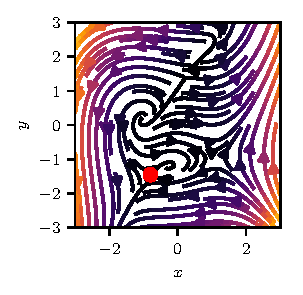
\includegraphics[width=.75\textwidth]{fixed_points_1}

			{\small Phase plane of the nonlinear system considered.}
		\end{minipage}%
		\hfill
		\begin{minipage}{.48\textwidth}
			\begin{itemize}
				\item The first fixed point is given by
				$${\bm x}^* = \begin{bmatrix} -0.798 & -1.449 \end{bmatrix}^T$$

				\bigskip

				\item The corresponding Jacobian matrix reads
				$${\bm J} = \begin{bmatrix} -1.03 & 1.78 \\ 0.91 & 0.2 \end{bmatrix}$$
			\end{itemize}
		\end{minipage}

		\vspace{1cm}
\end{frame}

\begin{frame}[t, c]{Second-order systems}{Fixed point n\textsuperscript{o}1}
		\begin{minipage}{.48\textwidth}
			\begin{itemize}
				\item ${\bm J}$ has two reals eigenvalues of opposite sign:
				$$\lambda_1 = 0.99 \text{ and } \lambda_2 = -1.83$$

				\item Such a fixed point is called a \alert{\textbf{saddle}}.
				\begin{itemize}
					\item[$\hookrightarrow$] Its first eigendirection ${\bm v}_1$ is repulsive while its second, ${\bm v}_2$, is attractive.
				\end{itemize}
			\end{itemize}
		\end{minipage}%
		\hfill
		\begin{minipage}{.48\textwidth}
			\centering
			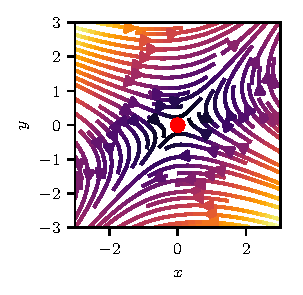
\includegraphics[width=.75\textwidth]{fixed_points_1_bis}

			{\small Trajectories in the vicinity of the fixed point ${\bm x}^*_1$.}
		\end{minipage}

		\vspace{1cm}
\end{frame}


\begin{frame}[t, c]{Second-order systems}{Fixed point n\textsuperscript{o}2}
		\begin{minipage}{.48\textwidth}
			\centering
			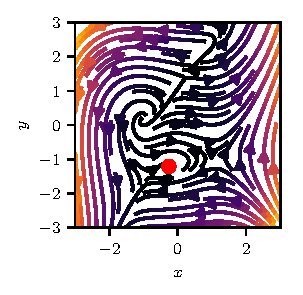
\includegraphics[width=.75\textwidth]{fixed_points_2}

			{\small Phase plane of the nonlinear system considered.}
		\end{minipage}%
		\hfill
		\begin{minipage}{.48\textwidth}
			\begin{itemize}
				\item The first fixed point is given by
				$${\bm x}^* = \begin{bmatrix} -0.26 & -1.2 \end{bmatrix}^T$$

				\bigskip

				\item The corresponding Jacobian matrix reads
				$${\bm J} = \begin{bmatrix} -0.69 & 2.05 \\ -0.79 & 0.2 \end{bmatrix}$$
			\end{itemize}
		\end{minipage}

		\vspace{1cm}
\end{frame}

\begin{frame}[t, c]{Second-order systems}{Fixed point n\textsuperscript{o}2}
		\begin{minipage}{.48\textwidth}
			\begin{itemize}
				\item ${\bm J}$ has complex conjugate eigenvalues:
				$$\lambda_{1, 2} = -0.24 \pm 1.2 i$$

				\item Such a fixed point is called a \alert{\textbf{spiral}}.
				\begin{itemize}
					\item[$\hookrightarrow$] In this case, $\Re(\lambda)<0$, so it is a spiral sink.
				\end{itemize}
			\end{itemize}
		\end{minipage}%
		\hfill
		\begin{minipage}{.48\textwidth}
			\centering
			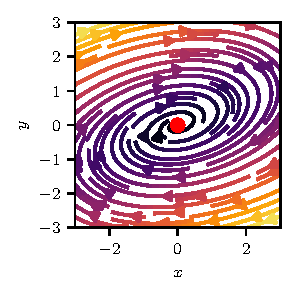
\includegraphics[width=.75\textwidth]{fixed_points_2_bis}

			{\small Trajectories in the vicinity of the fixed point ${\bm x}^*_1$.}
		\end{minipage}

		\vspace{1cm}
\end{frame}

\begin{frame}[t, c]{Second-order systems}{Classifying the fixed points}
	\begin{itemize}
		\item For a $2 \times 2$ matrix, its eigenvalues are solution of
		$$\lambda^2 - \trace({\bm L}) \lambda + \det({\bm L}) = 0,$$
		where $\trace({\bm L}) = l_{11} + l_{22}$ and $\det({\bm L}) = l_{11}l_{22} - l_{21}l_{12}$.

		\bigskip

		\item All the different types of fixed points can be placed onto a $\trace({\bm L})$--$\det({\bm L})$ diagram.
	\end{itemize}

	\vspace{1cm}
\end{frame}

\begin{frame}[t, c]{Second-order systems}{Classifying the fixed points}
	\vspace{-0.5cm}
	\centering
	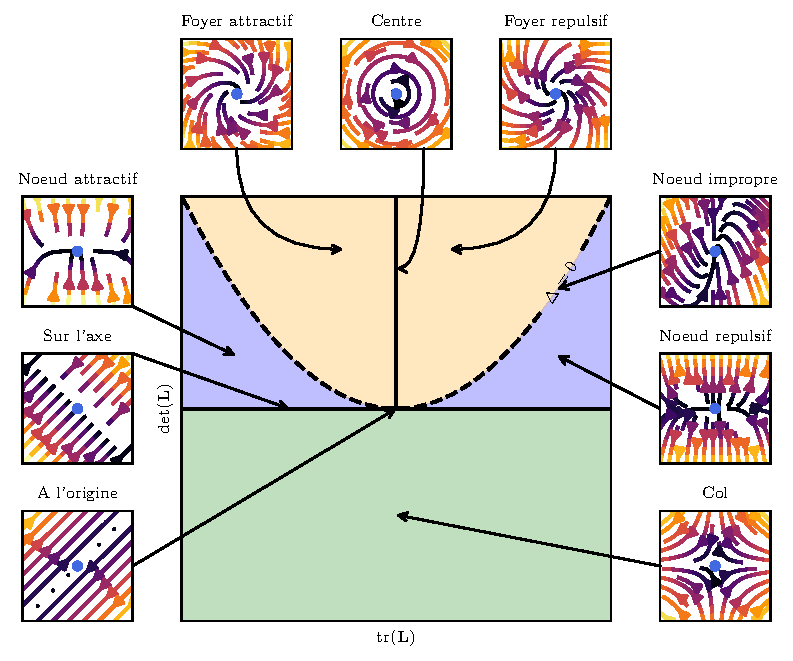
\includegraphics[height=.8\textheight]{fixed_points_classification}

\end{frame}

\end{document}
